\documentclass[8pt,sans,mathserif,aspectratio=43]{beamer}

\usepackage{ucs}
\usepackage[T1]{fontenc}
\usepackage[utf8x]{inputenc}

\usepackage{kerkis}
% \usepackage{eulervm}
% \usepackage{courier}
% \usepackage{palatino}
% \usepackage{kmath}

\usepackage{time}
\usepackage{graphicx}
\usepackage{color}
\usepackage{amssymb,amsmath}
\usepackage{isomath}
\hypersetup{unicode}

% Beamer setup

\usetheme{default}
\useoutertheme{infolines-center}
\usecolortheme{whale}

\definecolor{blendedblue}{rgb}{0.037,0.366,0.551}

\setbeamercolor{structure}{fg=blendedblue}
\setbeamercolor{titlelike}{parent=structure}
\setbeamercolor{frametitle}{fg=black}
\setbeamercolor{title}{fg=black}
\setbeamercolor{item}{fg=black}

% \setbeamercovered{transparent}
\setbeamercovered{invisible}

\setbeamertemplate{footline}{}
\setbeamertemplate{navigation symbols}{}

\defbeamertemplate*{title page}{customized}[1][]
{\centering{
    \vfill
    \usebeamerfont{title}\inserttitle\par
    \vfill
    \usebeamerfont{subtitle}\usebeamercolor[fg]{subtitle}\insertsubtitle\par
    \vfill
    \usebeamercolor[fg]{titlegraphic}\inserttitlegraphic
    \vfill
    \usebeamerfont{author}\insertauthor\par
    \vfill
    \usebeamerfont{institute}\insertinstitute\par
    \vfill
    \usebeamerfont{date}\insertdate\par
    \vfill
  }
}

% New commands-environments

\newcommand {\framedgraphic}[3]{
  \begin{frame}{#1}
    \begin{center}
      \includegraphics[width=\textwidth, keepaspectratio]
      {#2}\let\thefootnote\relax\footnote{#3}
    \end{center}
  \end{frame}
}

\newcommand{\spacer}[0]{
  \vspace{5pt}}

\begin{document}

\title{Simulation of Tsunami impact upon Coastline}
\titlegraphic{\includegraphics[width=0.8\textwidth]{figures/paraview.png}}
\author{A. Spathis-Papadiotis, K. Moustakas} \institute{ECE Department,
  University of Patras} \date{June 15, 2016}

%%%%%%%%%%%%%%%%%%%%%%%%%%%%%%%%%%%%%%%%%%%%%%%%%%%%%%%%%%%%%%%%%%%%%%%%%%%%%%%%

\begin{frame}
  \titlepage
\end{frame}

%%%%%%%%%%%%%%%%%%%%%%%%%%%%%%%%%%%%%%%%%%%%%%%%%%%%%%%%%%%%%%%%%%%%%%%%%%%%%%%%

\section{Introduction}

\begin{frame}{Generation of a Tsunami}
  \includegraphics[width=0.5\textwidth]{figures/tsunami-gen-0.pdf}
  \includegraphics[width=0.5\textwidth]{figures/tsunami-gen-1.pdf}\\
  \includegraphics[width=0.5\textwidth]{figures/tsunami-gen-2.pdf}
  \includegraphics[width=0.5\textwidth]{figures/tsunami-gen-3.pdf}
  \let\thefootnote\relax\footnote{From U.S. Geological Survey, Circular 1187}
\end{frame}

%%%%%%%%%%%%%%%%%%%%%%%%%%%%%%%%%%%%%%%%%%%%%%%%%%%%%%%%%%%%%%%%%%%%%%%%%%%%%%%%

\framedgraphic{} {figures/tsunami-hit.jpg} {From \texttt{www.theatlantic.com}}

%%%%%%%%%%%%%%%%%%%%%%%%%%%%%%%%%%%%%%%%%%%%%%%%%%%%%%%%%%%%%%%%%%%%%%%%%%%%%%%%

\section{Framework}

\begin{frame}{SPH Advantages}
  \begin{itemize}
  \item Inherent conservation of many important system quantities like mass,
    momentum, energy.\pause
  \item Exact, isotropic and invariable treatment of pure advection in every
    inertial frame of reference.\pause
  \item Dynamic adaptivity of resolution and computational load to simulation
    space and time.\pause
  \item Natural treatment of boundary conditions and special interactions in
    multiphase/multicomponent applications through particle interactions.
  \end{itemize}
  \includegraphics[width=\textwidth]{figures/boundary-particles.pdf}
  \only<4>{\let\thefootnote\relax\footnote{Figure from Akinci et al., 2012}}
\end{frame}

%%%%%%%%%%%%%%%%%%%%%%%%%%%%%%%%%%%%%%%%%%%%%%%%%%%%%%%%%%%%%%%%%%%%%%%%%%%%%%%%

\begin{frame}{SPH Formulation}
  The central notion of SPH is the spatially weighted interpolation:
  \begin{equation*}
    A(\vec{r}) = \sum_i \frac{m_i}{\rho_i} A(\vec{r}_i) W(\vec{r}-\vec{r}_i, h)
  \end{equation*}
  \pause The pressure gradient and velocity laplacian are needed for the
  calculation of pressure and viscosity forces:
  \begin{equation*}
    \nabla P = \sum_i \frac{m_i}{\rho_i} P \nabla W(\vec{r} - \vec{r}_i, h)
    \hspace{20pt}
    \nabla^2\vec{v} = \sum_i \frac{m_i}{\rho_i} (\vec{v}_i - \vec{v}) \nabla^2
    W(\vec{r}-\vec{r}_i, h)
  \end{equation*}
  \pause Pressure gradient is symmetrized by using a different estimator,
  derived from the gradient product rule:
  \begin{equation*}
    \nabla P = \rho \sum_i m_i \left(\frac{P}{\rho^2} + \frac{P_i}{\rho_i^2} \right)
    \nabla W(\vec{r}-\vec{r}_i, h)
  \end{equation*}
  \pause
  \begin{center}
    \vspace{-25pt}
    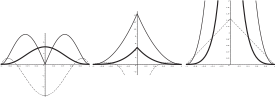
\includegraphics[width=0.8\textwidth]{figures/smoothing-kernels.pdf}\\
    \vspace{-10pt}
  \end{center}
  \hspace{66pt} Density \hspace{66pt} Pressure \hspace{66pt} Viscosity
  \only<4>{\let\thefootnote\relax\footnote{Figure from M{\"u}ller et al., 2003}}
\end{frame}

%%%%%%%%%%%%%%%%%%%%%%%%%%%%%%%%%%%%%%%%%%%%%%%%%%%%%%%%%%%%%%%%%%%%%%%%%%%%%%%%

\section{Implementation}

\begin{frame}{Architecture}
  \begin{center}
    \includegraphics[width=0.9\textwidth, keepaspectratio]{figures/architecture.pdf}
  \end{center}
\end{frame}

%%%%%%%%%%%%%%%%%%%%%%%%%%%%%%%%%%%%%%%%%%%%%%%%%%%%%%%%%%%%%%%%%%%%%%%%%%%%%%%%

\begin{frame}{SPH Engine \textendash\ LP grid}
  SPH Engine calculates fluid forces according to SPH:\\ \vspace{5pt}
  \begin{tabular}{rll}
    Density $\rightarrow$ State Equation $\rightarrow$ Pressure $\rightarrow$
    Pressure Gradient & $\Rightarrow$ & Pressure Forces\\
    Velocity $\rightarrow$ Velocity Laplacian & $\Rightarrow$ & Viscosity Forces\\
  \end{tabular}\\ \vspace{5pt}
  which are integrated back to the particle system through Bullet.\\\pause
  \vspace{5pt}
  Spatial hashing data structure (LP grid) for the optimization of particle
  access:
  \begin{center}
    \includegraphics[width=0.9\textwidth]{figures/lp-grid.pdf}
  \end{center}\pause
  \begin{itemize}
  \item Cohesive particle storage.\pause
  \item Fast $O(1)$, hash table access onto continuous memory.\pause
  \item Quick, in-place update, with no memory (re-)allocation needed.\pause
  \item Optimized cache memory usage during particle interaction scanning owing
    to the LUT-encoded locality preserving mapping from the 3D domain to linear
    storage, obtained by spatial sorting of the grid cells.
  \end{itemize}
\end{frame}

%%%%%%%%%%%%%%%%%%%%%%%%%%%%%%%%%%%%%%%%%%%%%%%%%%%%%%%%%%%%%%%%%%%%%%%%%%%%%%%%

\begin{frame}{Performance}
  \begin{center}
    \includegraphics[width=\textwidth]{figures/performance-pt.pdf}
  \end{center}
\end{frame}

%%%%%%%%%%%%%%%%%%%%%%%%%%%%%%%%%%%%%%%%%%%%%%%%%%%%%%%%%%%%%%%%%%%%%%%%%%%%%%%%

\section{Results}

\subsection{Fluid}

\begin{frame}{Interactive visualization}
  \includegraphics[width=\textwidth]{figures/paraview.png}
\end{frame}

%%%%%%%%%%%%%%%%%%%%%%%%%%%%%%%%%%%%%%%%%%%%%%%%%%%%%%%%%%%%%%%%%%%%%%%%%%%%%%%%

\begin{frame}{Pressure}
  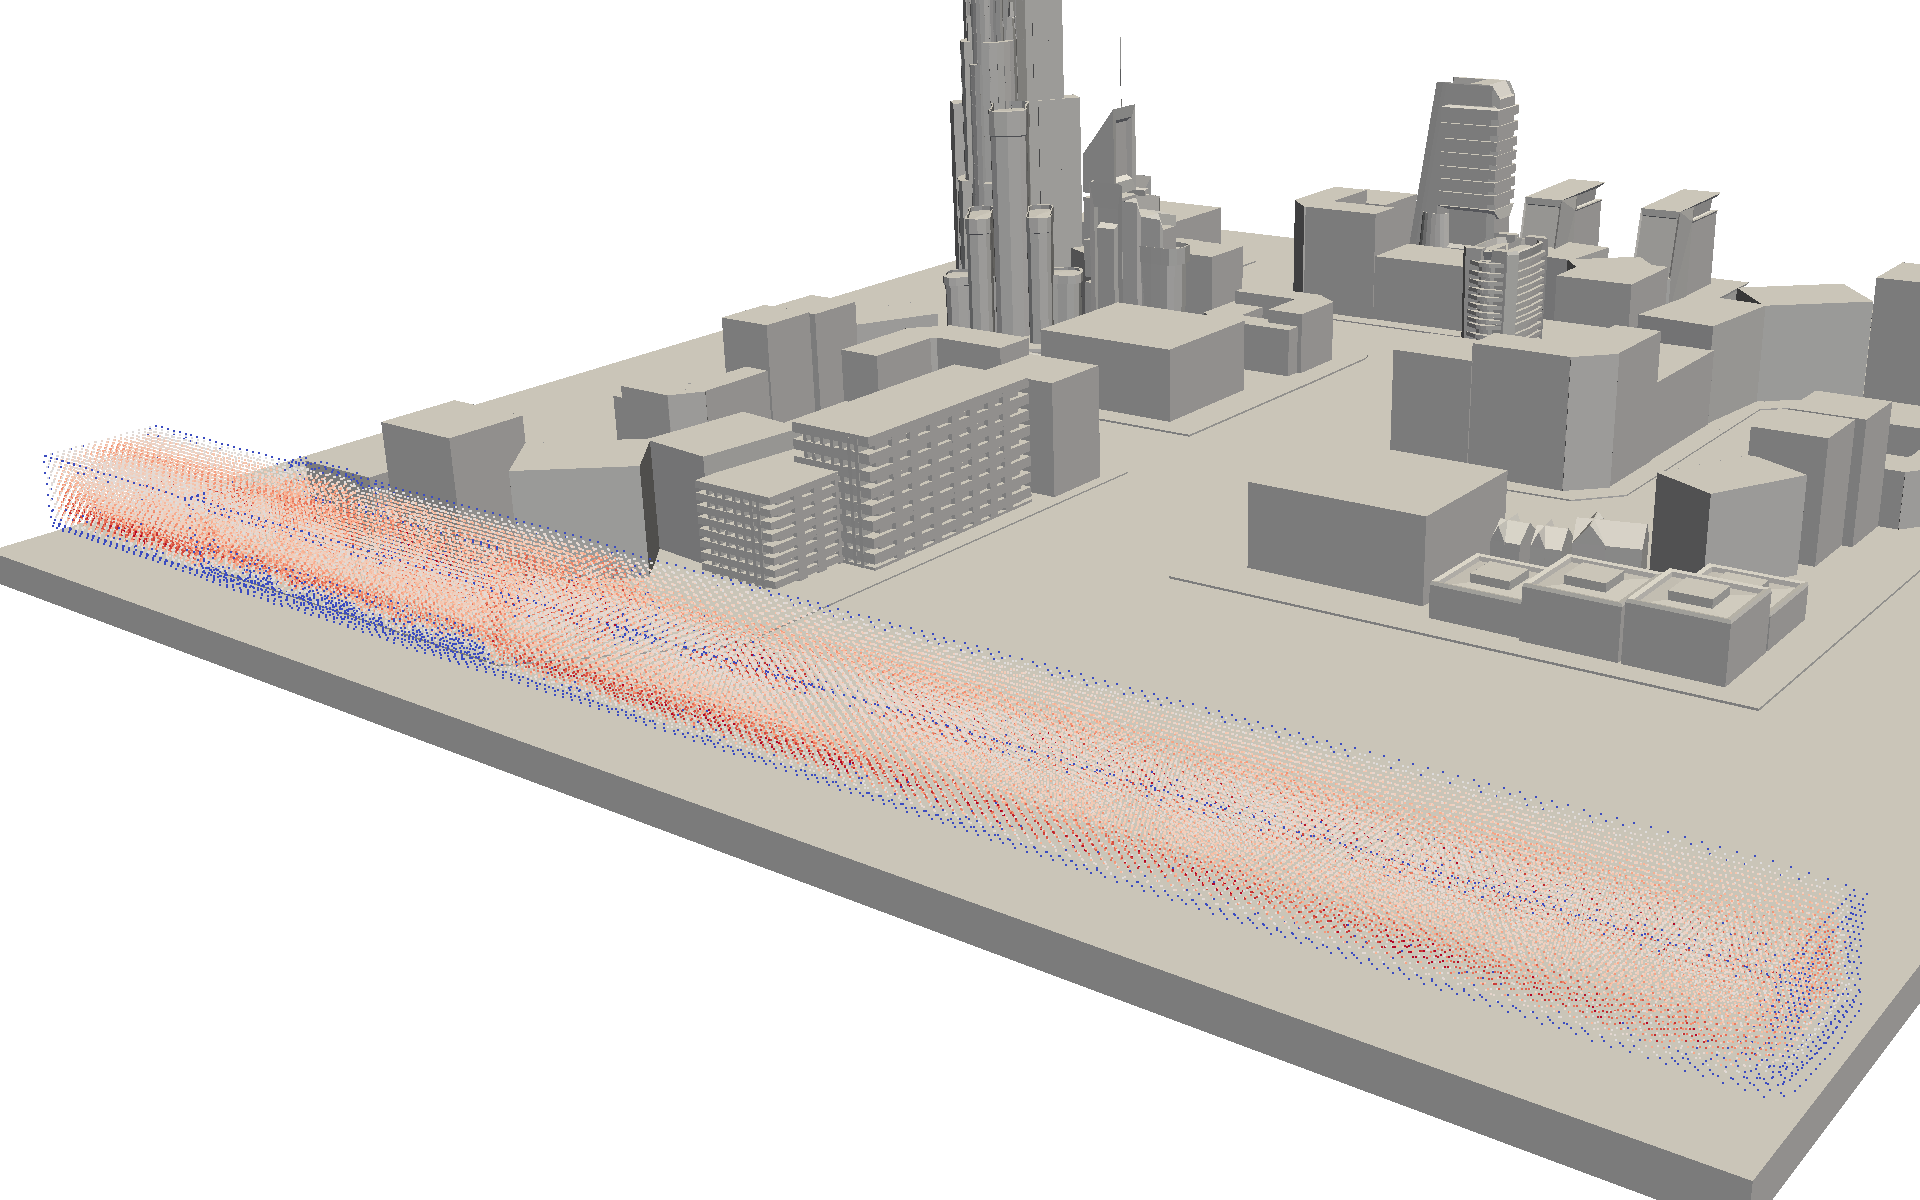
\includegraphics[width=.5\textwidth]{figures/press-0.png}
  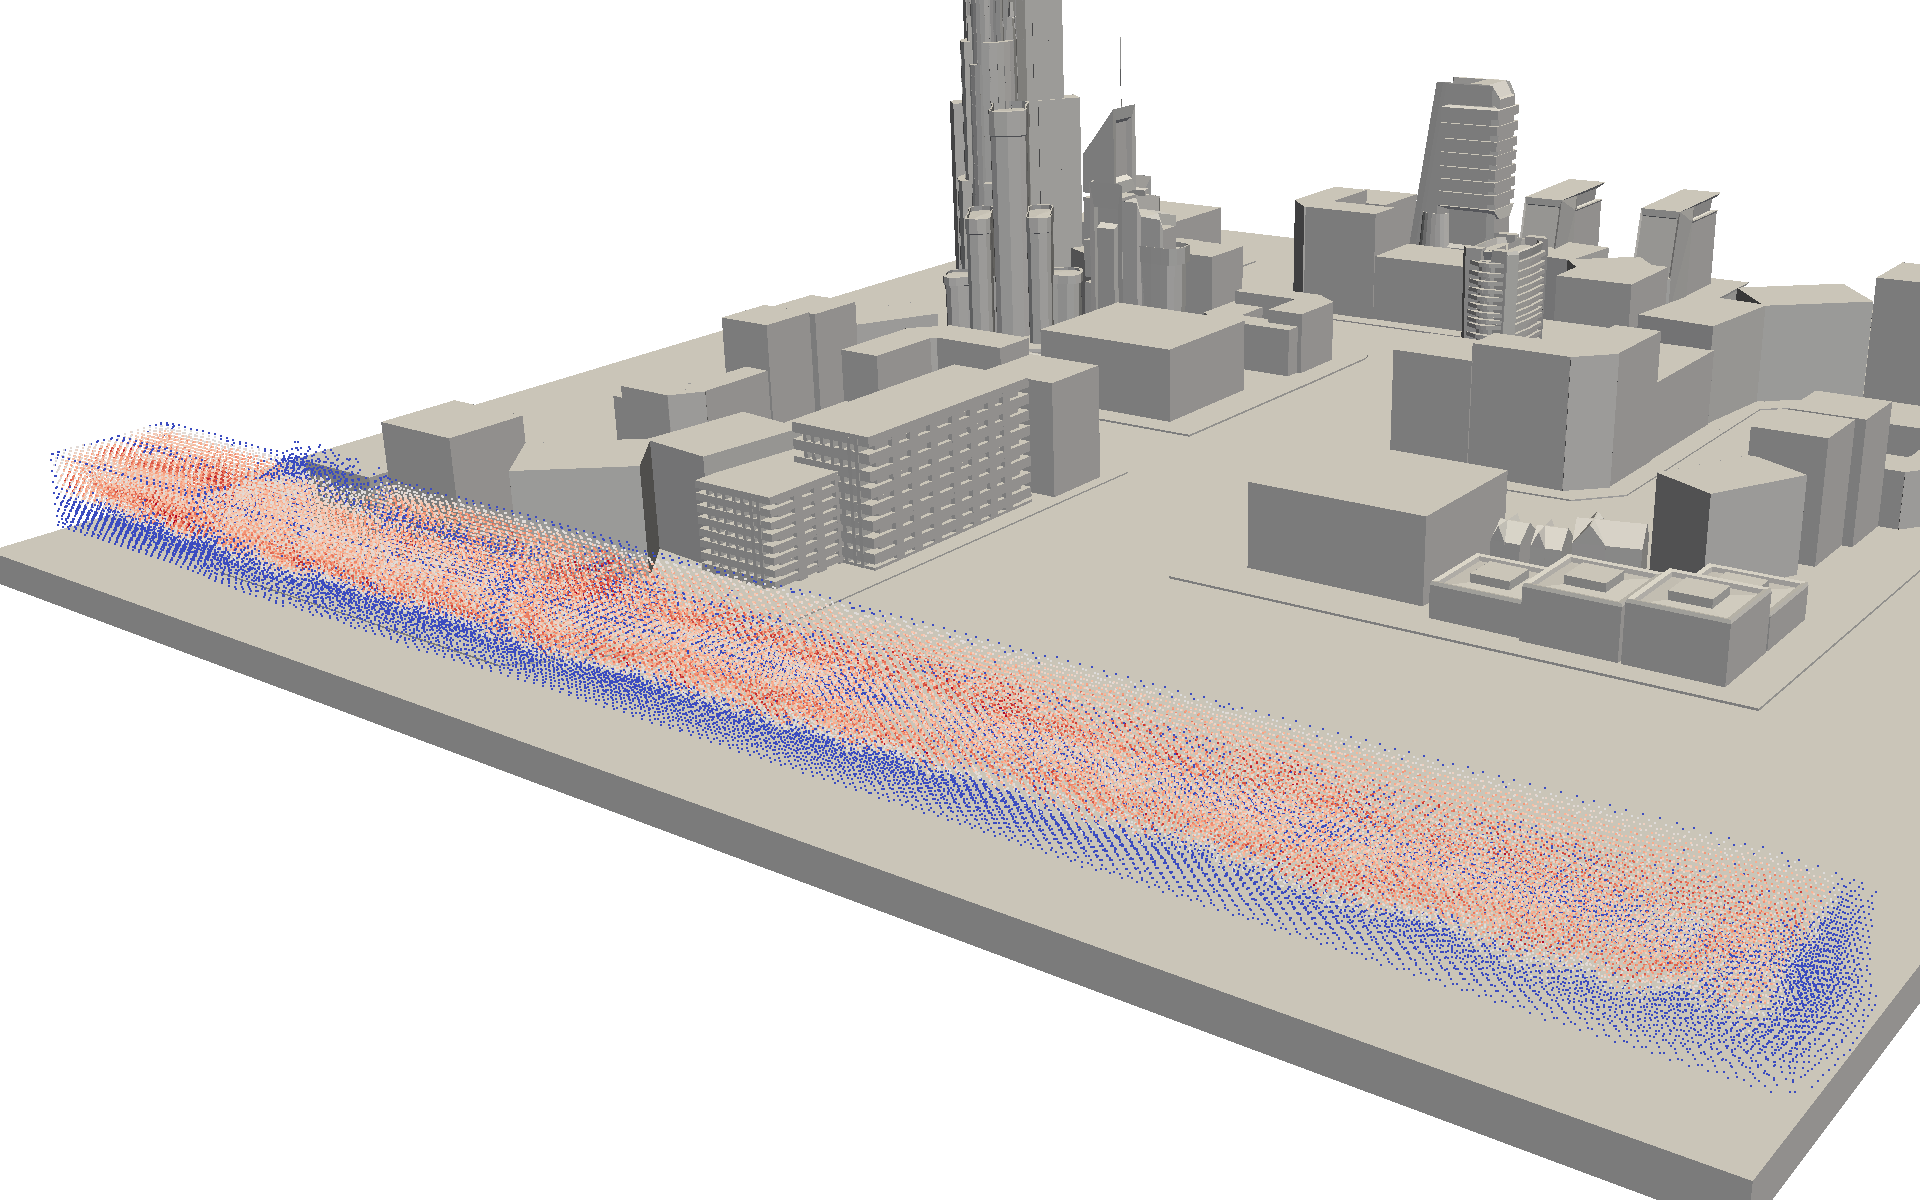
\includegraphics[width=.5\textwidth]{figures/press-1.png}\\
  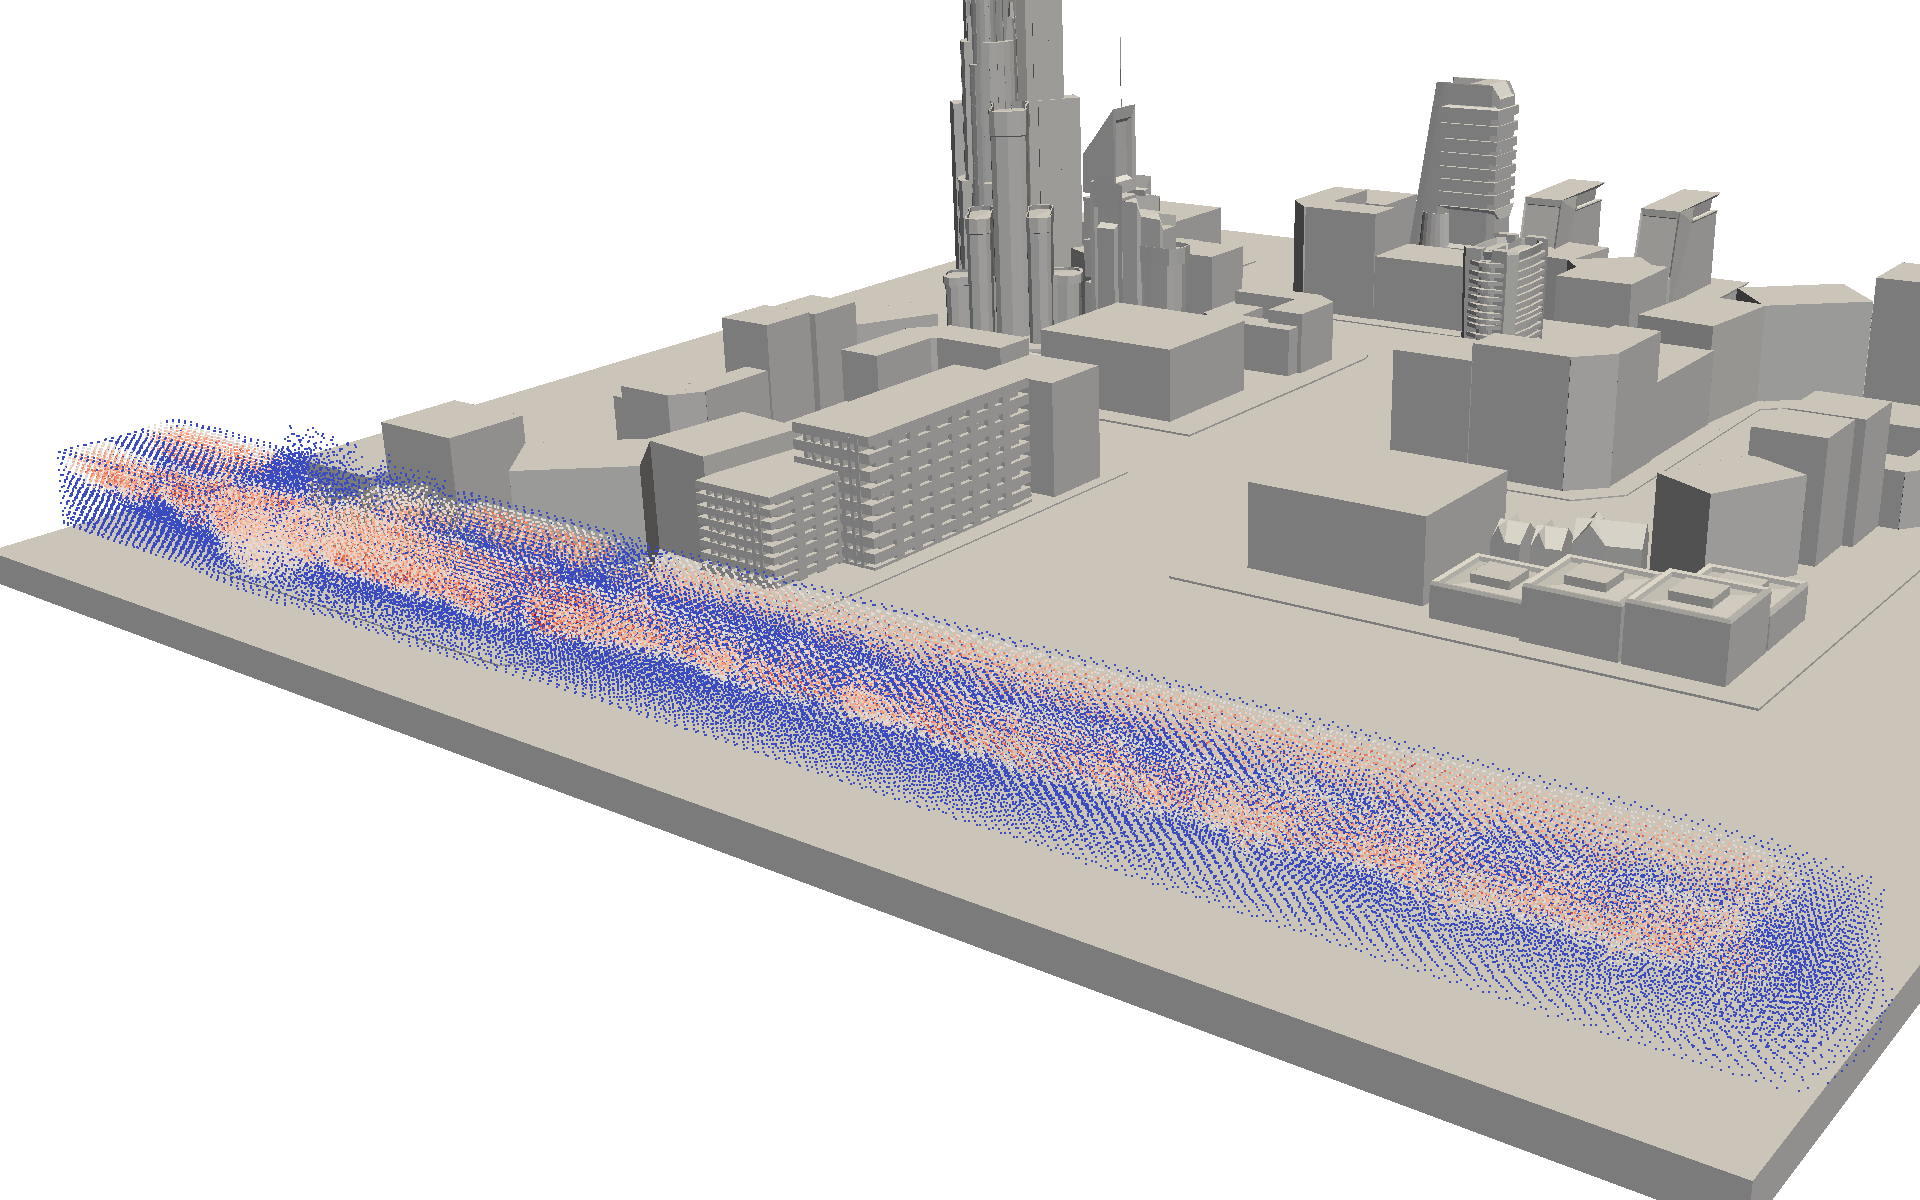
\includegraphics[width=.5\textwidth]{figures/press-2.png}
  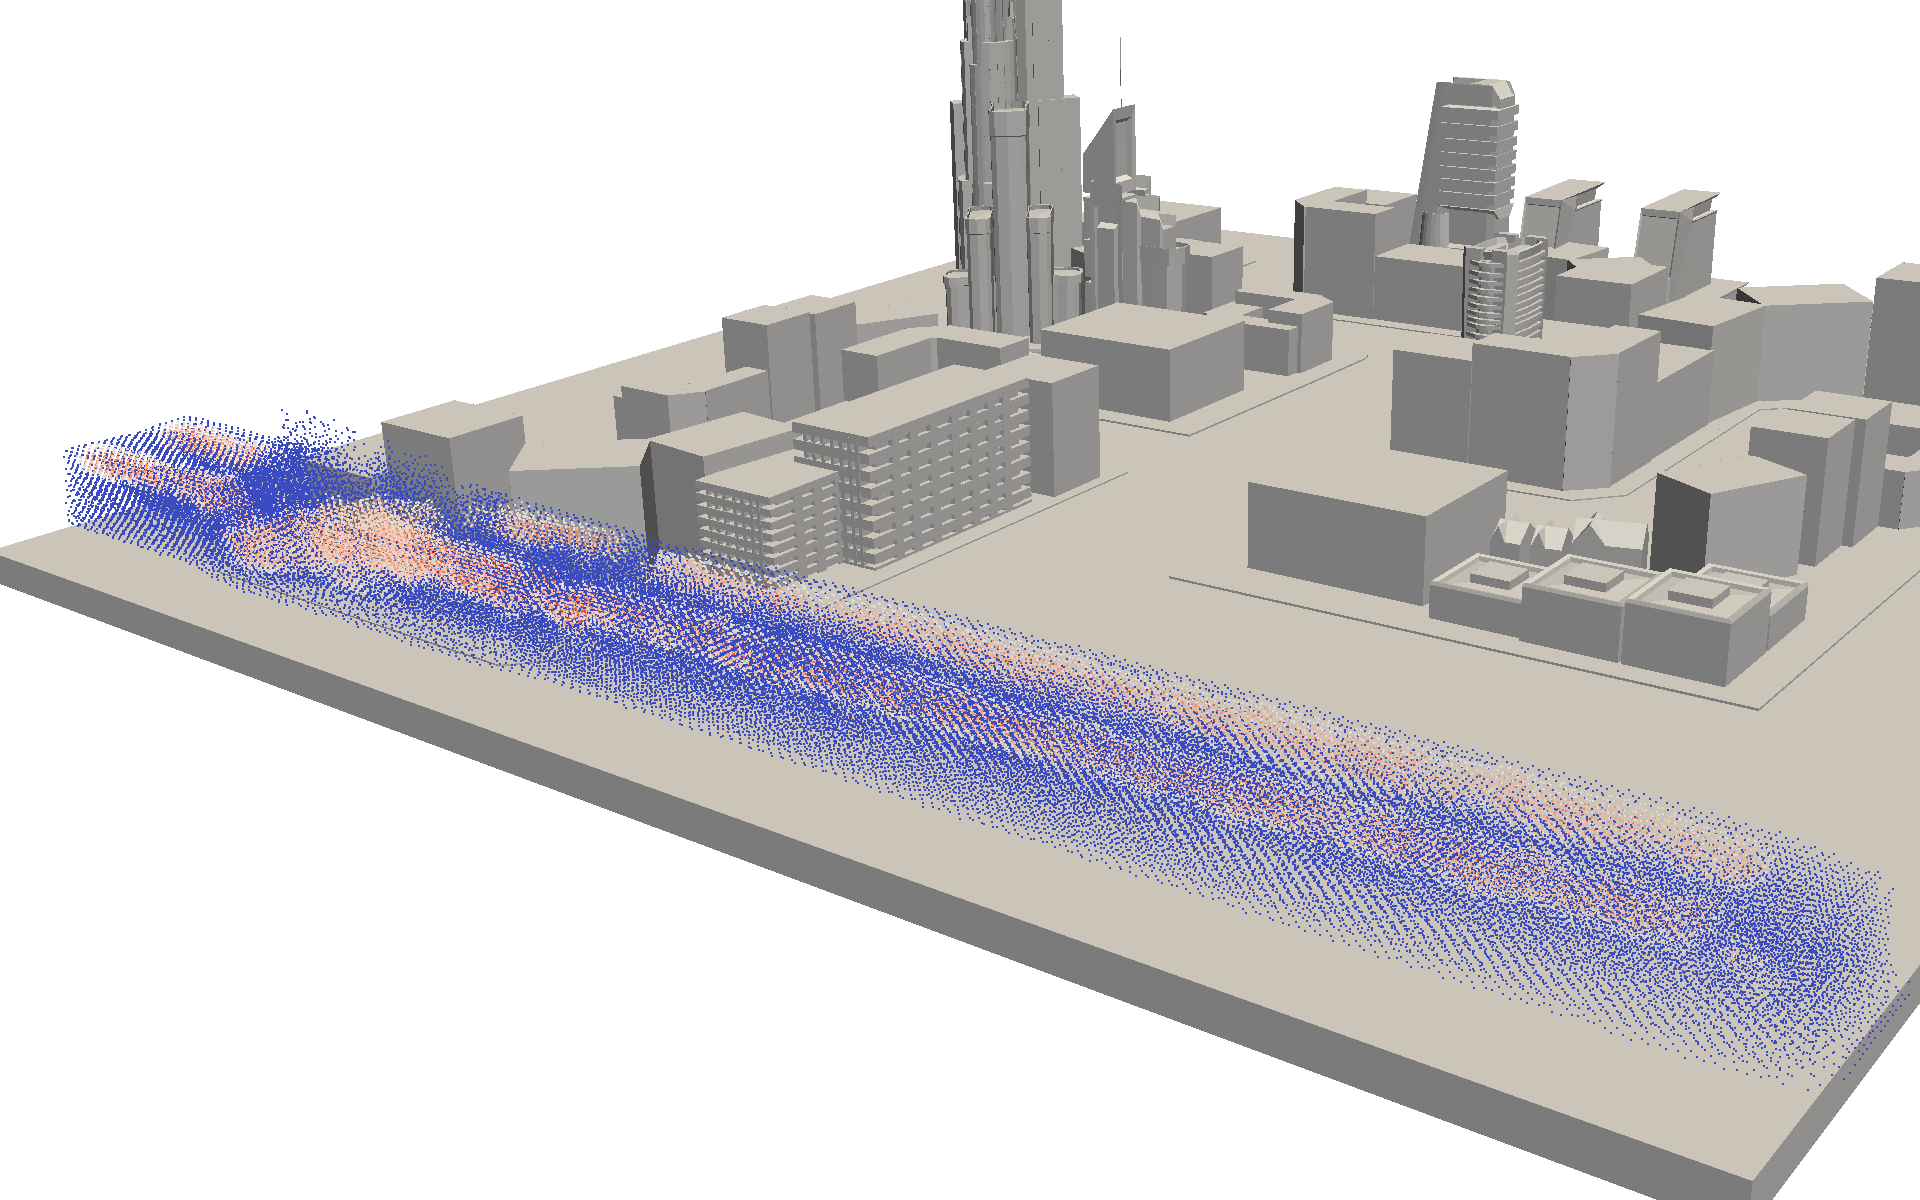
\includegraphics[width=.5\textwidth]{figures/press-3.png}
\end{frame}

%%%%%%%%%%%%%%%%%%%%%%%%%%%%%%%%%%%%%%%%%%%%%%%%%%%%%%%%%%%%%%%%%%%%%%%%%%%%%%%%

\begin{frame}{Viscosity}
  \includegraphics[width=.5\textwidth]{figures/visc-0.png}
  \includegraphics[width=.5\textwidth]{figures/visc-1.png}\\
  \includegraphics[width=.5\textwidth]{figures/visc-2.png}
  \includegraphics[width=.5\textwidth]{figures/visc-3.png}
\end{frame}

%%%%%%%%%%%%%%%%%%%%%%%%%%%%%%%%%%%%%%%%%%%%%%%%%%%%%%%%%%%%%%%%%%%%%%%%%%%%%%%%

\begin{frame}{Neighbour particle count}
  \includegraphics[width=\textwidth]{figures/samples.png}
\end{frame}

%%%%%%%%%%%%%%%%%%%%%%%%%%%%%%%%%%%%%%%%%%%%%%%%%%%%%%%%%%%%%%%%%%%%%%%%%%%%%%%%

\subsection{Coastline}

\begin{frame}{Impulses}
  \includegraphics[width=.5\textwidth]{figures/impulses-0.png}
  \includegraphics[width=.5\textwidth]{figures/impulses-1.png}\\
  \includegraphics[width=.5\textwidth]{figures/impulses-2.png}
  \includegraphics[width=.5\textwidth]{figures/impulses-3.png}
\end{frame}

%%%%%%%%%%%%%%%%%%%%%%%%%%%%%%%%%%%%%%%%%%%%%%%%%%%%%%%%%%%%%%%%%%%%%%%%%%%%%%%%

\begin{frame}{Impulse heatmap}
  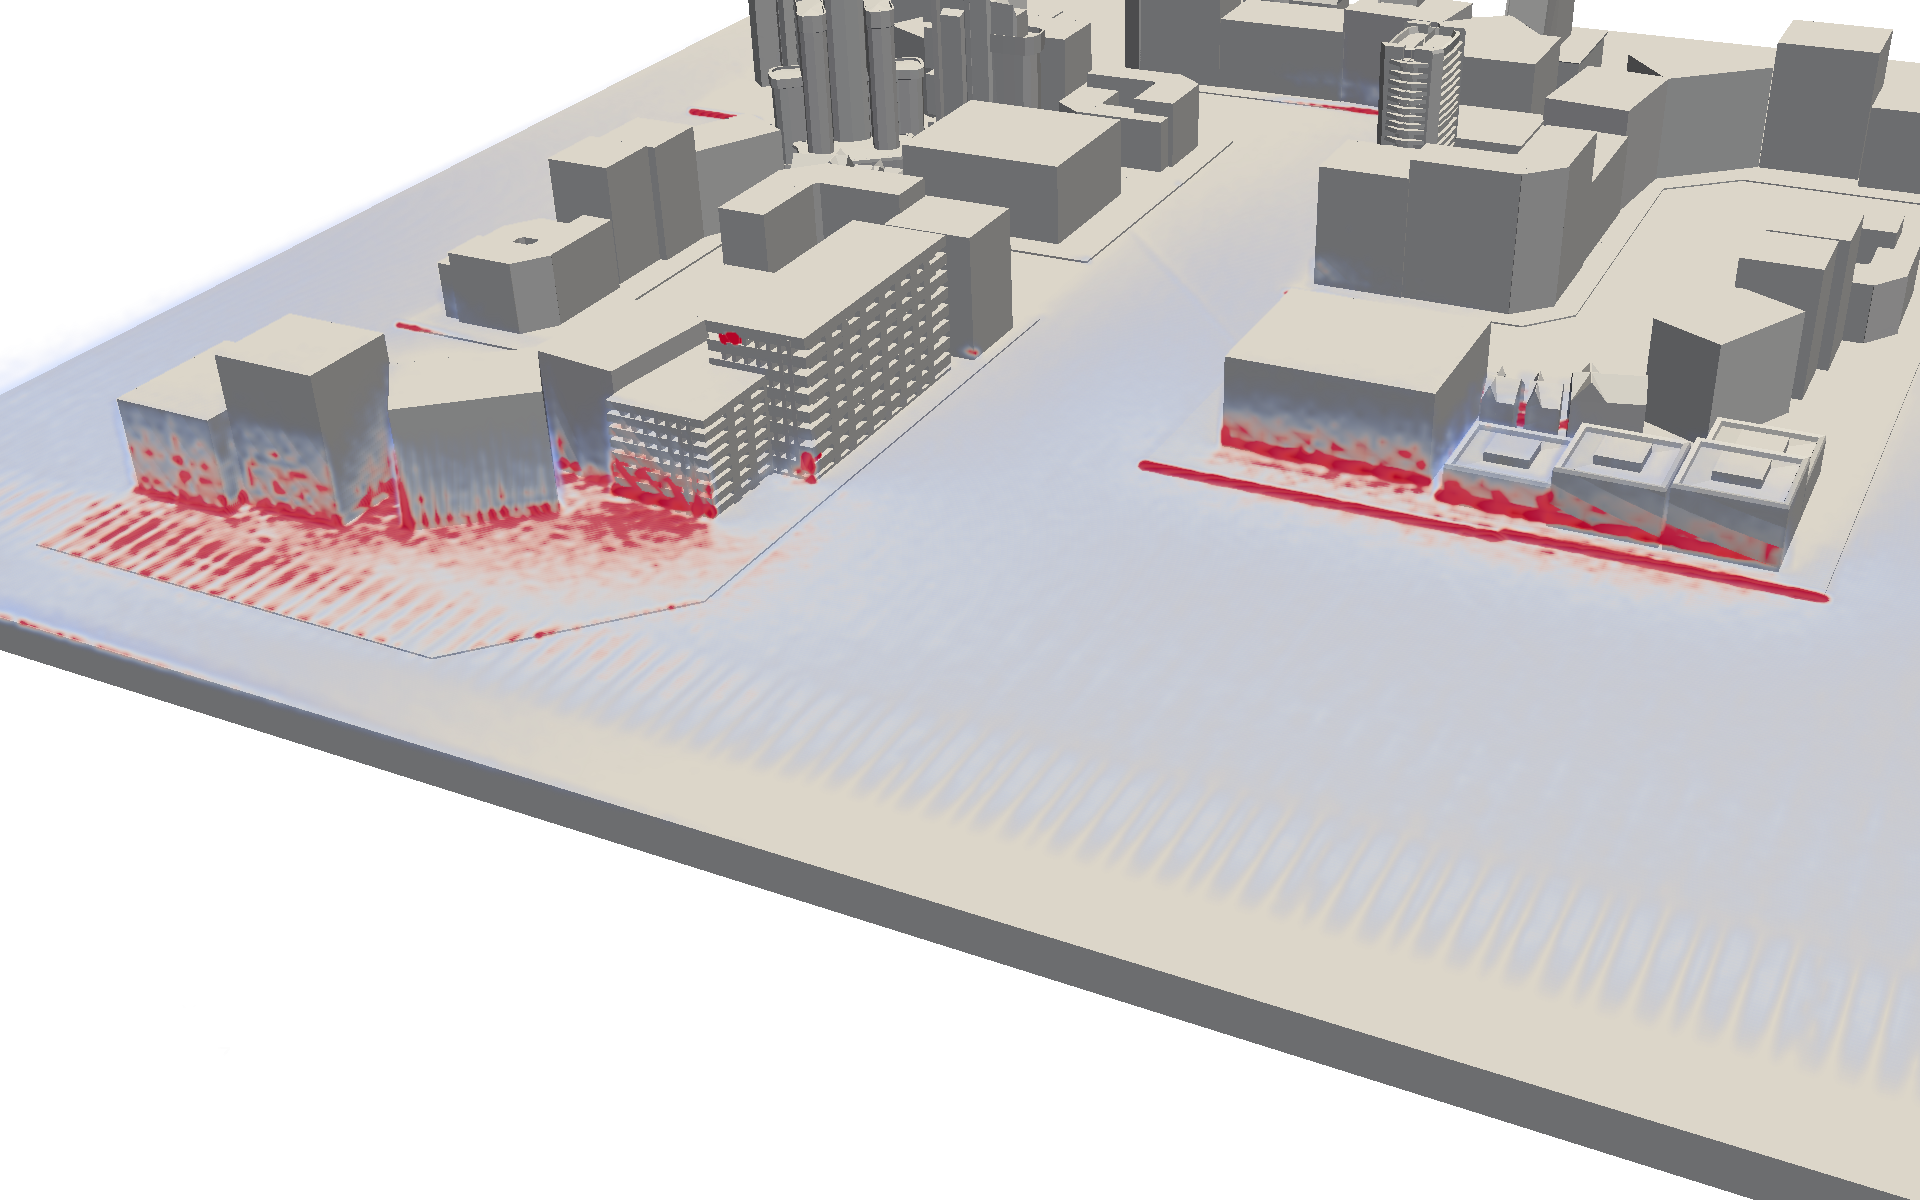
\includegraphics[width=\textwidth]{figures/impulse-heatmap-0.png}
\end{frame}

%%%%%%%%%%%%%%%%%%%%%%%%%%%%%%%%%%%%%%%%%%%%%%%%%%%%%%%%%%%%%%%%%%%%%%%%%%%%%%%%

\begin{frame}{Impulse heatmap}
  \includegraphics[width=\textwidth]{figures/impulse-heatmap-1.png}
\end{frame}

%%%%%%%%%%%%%%%%%%%%%%%%%%%%%%%%%%%%%%%%%%%%%%%%%%%%%%%%%%%%%%%%%%%%%%%%%%%%%%%%

\begin{frame}{Impulse heatmap}
  \includegraphics[width=\textwidth]{figures/impulse-heatmap-2.png}
\end{frame}

%%%%%%%%%%%%%%%%%%%%%%%%%%%%%%%%%%%%%%%%%%%%%%%%%%%%%%%%%%%%%%%%%%%%%%%%%%%%%%%%

\begin{frame}{Seawall effectiveness}
  \includegraphics[width=\textwidth]{figures/if-city0-free.png}\\
  \includegraphics[width=\textwidth]{figures/if-city0-seawall.png}
\end{frame}


%%%%%%%%%%%%%%%%%%%%%%%%%%%%%%%%%%%%%%%%%%%%%%%%%%%%%%%%%%%%%%%%%%%%%%%%%%%%%%%%

\section{}
\subsection{}
\begin{frame}
  \begin{center}
    \spacer\spacer\spacer\spacer\spacer\spacer
    Thank you!\\
    \spacer\spacer\spacer\spacer\spacer\spacer
    Questions?
  \end{center}
\end{frame}

\end{document}

%%% Local Variables:
%%% mode: latex
%%% TeX-master: t
%%% End:
